\chapter{Økonomi}

\section{Priser og finansiering}
Dagligvarer er mye billigere enn hva man finner i Norge, det er rundt halv pris på det meste. Alkohol og tobakk er mye gunstigere, 
en 0,5 liter øl på byen koster rundt 23-30 kroner.
Priser på leie av leilighet varier i forhold til beliggenhet, størelse og tilstand, men for rundt 4000 kroner får man en sentral leilighet.

\begin{figure}[h]
\center
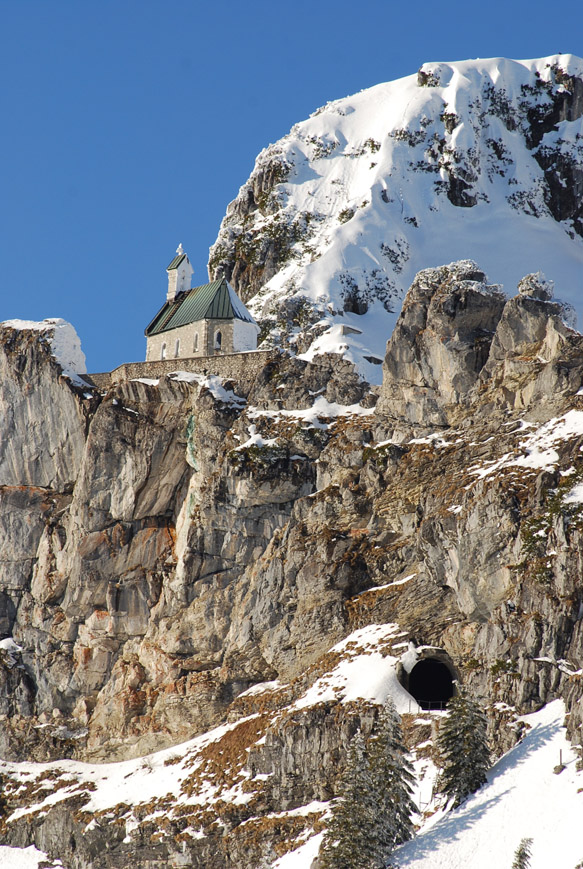
\includegraphics[width=0.2\textwidth]{./gfx/wendelstein}
\caption{Kirken på Wendelstein ligger høyest i Tyskland. Her er det meget god offpist-kjøring om vinteren.}
\end{figure}

\section{Lånekassen}
Du kan få støtte av lånekassen til å studere språk fra tre til fem mnd før studiestart. Dette kalles tilretteleggingssemester. Har du kommet inn på et studie kan du få språkstipend før studiestart .


 Du vil kunne få økonomisk støtte fra Lånekassen så lenge utdanningen din kan:
 
 
\begin{enumerate}
\item Utdanningen må tilsvare, være på nivå med, eller kan bli godkjent som en del av en norsk bachelor- eller mastergrad.
\item Lærestedet må være offisielt godkjent i studielandet.
\item Utdanningen må være på fulltid.
\end{enumerate}
 
 
Utdanningsstøtten er 90 800 kroner årlig og blir gitt som lån. 40 \% av støtten omgjøres til stipend forutsatt at alle eksamener er bestått (54 480 kroner er lån, 36 320 kroner er stipend).
Til høyere utdanning kan du få stipend til to tur-retur reiser, men ikke mer en 7250 kroner per studieår. Egenandelen er 2 080 kroner per studieår. 
Reisestipendet blir automatisk beregnet når du søker om stipend eller lån



\section{Privat stipend}
Se \url{http://www.legathandboken.no}. \\
Forskningsrådet deler hvert år ut stipender til studenter på som vil studere i Tyskland. Se Forskningsrådet for mer informasjon. \\
\url{www.forskningsradet.no}

\begin{figure}[h]
\center

\includegraphics[width=0.2\textwidth]{./gfx/russefest}
\caption{Haugalending på russefest ved Monopterosen i Englischer Garten}
\end{figure}

\section{Skolepenger}

I München betaler man skolepenger, men disse er svært lave og ligger på rundt 500 Euro. I tillegg må du betale en semesteravgift på mellom 50 og 200 Euro. Lånekassen gir utdannings- og skolepengestøtte til bachelor- og mastergrader ved offentlige godkjente læresteder for høyere utdanning i Tyskland. Du kan også få støtte til å ta deler av en norsk utdanning (utveksling) i Tyskland. For å få støtte fra Lånekassen, må du immatrikuleres som regulær student ved det tyske lærestedet.

Det er mulig at kravet om betaling av skolepenger vil frafalle i 2013/2014. Sjekk universitetets hjemmeside for informasjon om dette.


